\section{Busqueda de un dataset}
\label{sec:busquedaDataset}
Para poder entrenar modelos de \gls{ia} se requiere una gran cantidad de datos, en este caso de animaciones de los gestos escogidos que se han mencionado en la introducción.
Además, estos datos tienen que estar en un formato en el que se pueda extraer la información de los huesos (posición y rotación) para que pueda ser usado por los modelos, y tenían que ser compatibles con los huesos del traje de captura de movimiento.

\subsection{Dataset de la Universidad Carnegie Mellon}
La Universidad privada Carnegie Mellon, ubicada en Pittsburgh, Pensilvania, tiene dispoible de forma gratuita un dataset de movimientos recogidos mediante la captura de movimiento.\footnote{Enlace a la página del dataset de la Universidad Carnegie Mellon: \url{https://mocap.cs.cmu.edu/}}
Sin embargo este dataset no ha sido posible utilizarlo por tres motivos.

El primer motivo es la incompatibilidad del esqueleto utilizado por ellos con el utilizado por el traje de captura de movimiento Perception Neuron 3.
Como se puede ver en \cite{MCUINFO} su traje contiene 41 puntos usados para la captura, mostrados en la figura \ref{fig:MCUTraje}, dando a lugar al esqueleto mostrado en la figura \ref{fig:MCUEsqueleto}.

\begin{figure}[H]
    \centering
    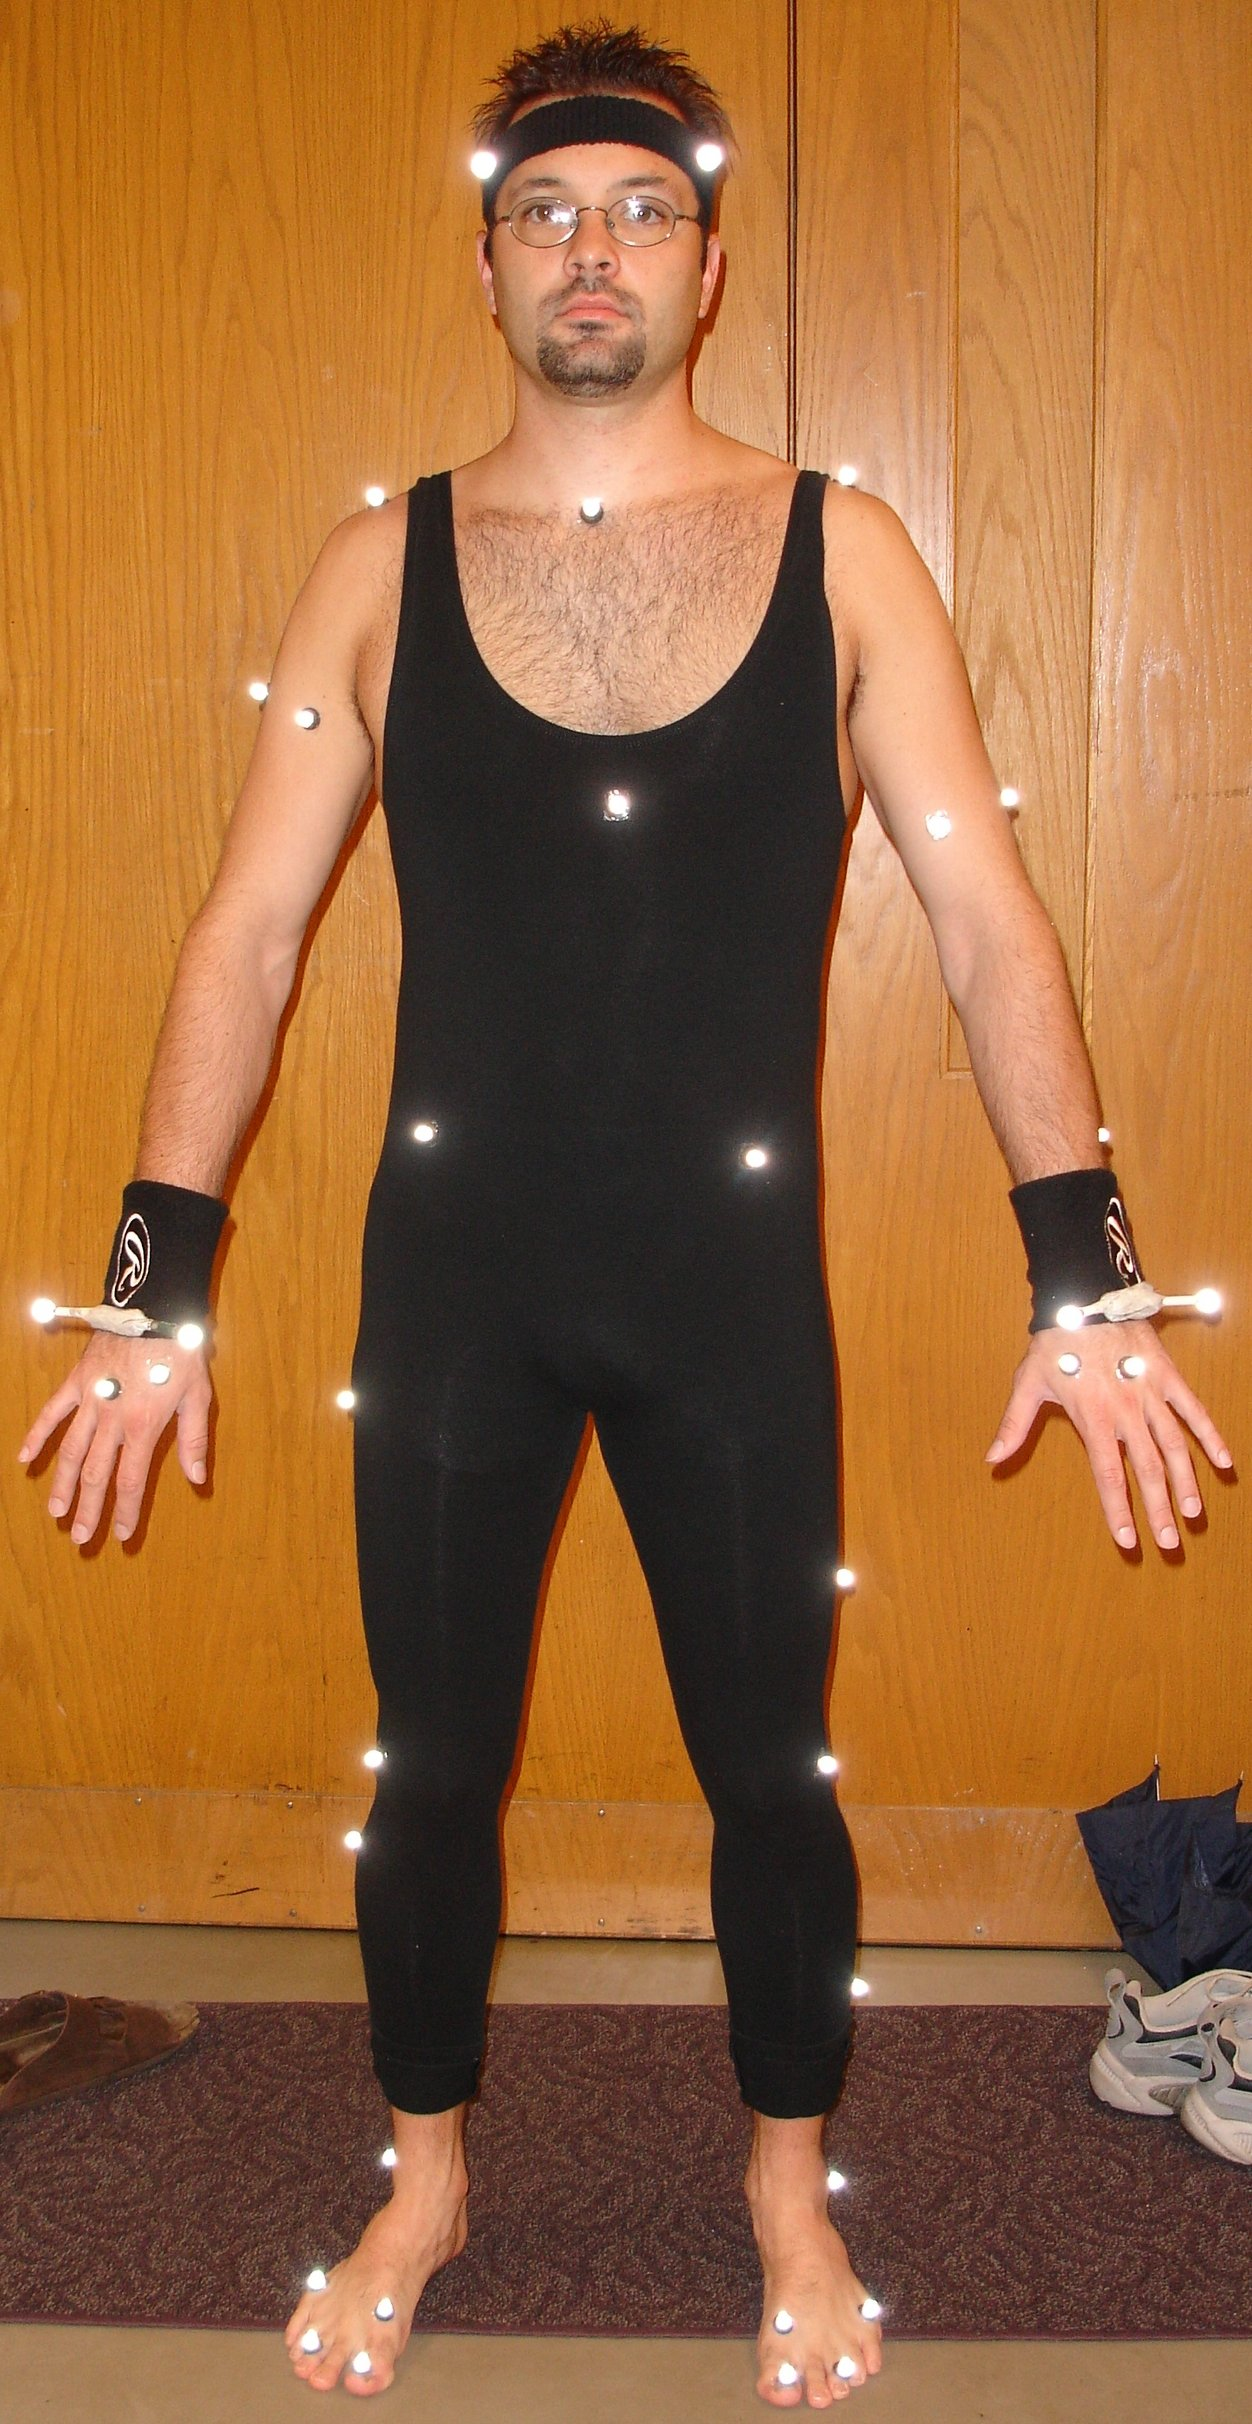
\includegraphics[width=0.3\textwidth]{Imagenes/Bitmap/MCUTraje.jpg}
    \caption{Imágen del traje de captura de movimiento usado para la base de datos de la Universidad Carnegie Mellon, Fuente: https://mocap.cs.cmu.edu/info.php}
    \label{fig:MCUTraje}
\end{figure}

\begin{figure}[H]
    \centering
    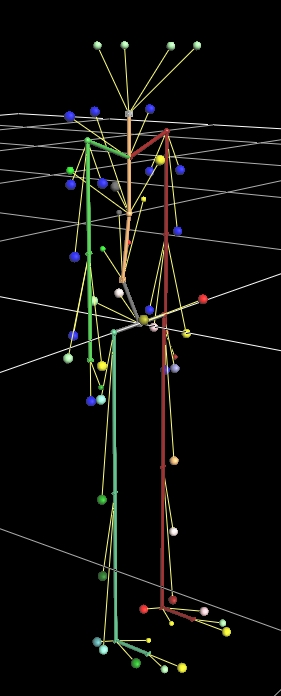
\includegraphics[width=0.23\textwidth]{Imagenes/Bitmap/MCUEsqueleto.jpg}
    \caption{Imágen del esqueleto resultante del traje de captura de movimiento usado por la Universidad Carnegie Mellon, Fuente: https://mocap.cs.cmu.edu/info.php}
    \label{fig:MCUEsqueleto}
\end{figure}

Por otro lado, como ya mencionamos en el capítulo \ref{sec:traje}, el traje Perception Neuron 3 contiene 17 puntos, haciendo incompatibles los esqueletos.

El segundo motivo por el que no se ha usado el dataset de la Universidad Carnegie Mellon es el formato de las animaciones disponibles.
Las animaciones presentes en el dataset vienen en tres formatos distintos: c3d, asf (o amc) y vsk (o v).
Los formatos c3d, vsk y v son unos formatos en binario usados para objetos en 3D, por lo que no se puede usar de forma sencilla para extraer la información del propio archivo.
Por otro lado los archivos asf y amc son archivos en formato ASCII con la información de los huesos. Sin embargo la documentación aportada para poder usar la información es incompleta.

El último motivo por el que no se ha usado este dataset es por la escasez de animaciones de los gestos buscados.
Animaciones como ``correr'' sí están presentes (aunque no en abundancia), pero otras como ``pelear'' o ``saludar'' no.

Este último problema también ha estado presente en páginas específicas de bancos de datasets como Kaggle.

\subsection{Kaggle}

TO DO: HABLAR DE LA ESCASEZ DE DATASET DE ANIMACIONES EN KAGGLE

TO DO: HABLAR DE POR QUÉ DESCARTAMOS IMÁGENES Y NOS CENTRAMOS MÁS EN ESQUELETOS

Ya que no se encontró un gran dataset que cumpliese con nuestros requerimientos se tomó la decisión de buscar en un banco de animaciones los gestos requeridos y transformar esas animaciones en un formato que puediesen ser procesados.